\documentclass{hipatia}
\usepackage[utf8]{inputenc}
\usepackage[brazil]{babel}
\usepackage{amssymb,amsthm,amsfonts,amsmath,pifont}
%\usepackage{dropping}
\usepackage{pstricks, graphicx, epsf}
\usepackage{caption}% para numerar as figuras com o captionof usando o begin{center}
\usepackage{multicol}% para duas colunas
\usepackage[makeroom]{cancel} %para usar o cancelamento.
\usepackage{yhmath}
\usepackage{graphicx} % Required for inserting images
\usepackage{pgf,tikz}
\usetikzlibrary{fit, shapes.geometric, arrows}
\usepackage{wasysym}
%\usepcakage{arcs}

\usepackage{lipsum}
\usepackage{makeidx}
\usepackage{pstricks}
\usepackage{graphicx}
\usepackage{hyperref}
\usepackage{version}
\usepackage{enumerate}
%Use \DeclareMathOperator para definir novos
% operadores para o modo matemático
\DeclareMathOperator{\sen}{sen}

%Evite numerar teoremas
%Prefira nomeá-los
%Use os ambientes abaixo
\newtheorem*{theorem*}{Teorema}
\newtheorem*{lemma*}{Lema}
\newtheorem{problem*}{Problema}
\newtheorem*{solution*}{Solução}


\subtitle{Problema}
\title{Contando Inversões}
\author{Yure Carneiro e Samuel Feitosa}
%\date{June 2025}
\let\widering\relax
\begin{document}
\setcounter{page}{\problemapage}
\maketitle



\section{Soluções da Edição Anterior}

\section{Problemas Universitários}

\begin{problem*}
No plano complexo (plano de Argand-Gauss) um 
quadrado $ABCD$ tem centro no ponto $z=0$. 
    \begin{center}
       % \includegraphics[scale=0.6]%{ElonComplexos.png}

\begin{tikzpicture}[x=0.75pt,y=0.75pt,yscale=-0.6,xscale=0.6]
%uncomment if require: \path (0,300); %set diagram left start at 0, and has height of 300

%Shape: Axis 2D [id:dp4855606947862082] 
\draw [color={rgb, 255:red, 73; green, 135; blue, 206 }  ,draw opacity=1 ][line width=1.5]  (4.27,150.3) -- (324,150.3)(154.27,3) -- (154.27,258.3) (317,145.3) -- (324,150.3) -- (317,155.3) (149.27,10) -- (154.27,3) -- (159.27,10)  ;
%Straight Lines [id:da78389926760332] 
\draw [color={rgb, 255:red, 0; green, 0; blue, 0 }  ,draw opacity=1 ][line width=1.5]    (125.88,50.18) -- (54.82,175.88) ;
\draw [shift={(54.82,175.88)}, rotate = 119.48] [color={rgb, 255:red, 0; green, 0; blue, 0 }  ,draw opacity=1 ][fill={rgb, 255:red, 0; green, 0; blue, 0 }  ,fill opacity=1 ][line width=1.5]      (0, 0) circle [x radius= 4.36, y radius= 4.36]   ;
\draw [shift={(125.88,50.18)}, rotate = 119.48] [color={rgb, 255:red, 0; green, 0; blue, 0 }  ,draw opacity=1 ][fill={rgb, 255:red, 0; green, 0; blue, 0 }  ,fill opacity=1 ][line width=1.5]      (0, 0) circle [x radius= 4.36, y radius= 4.36]   ;
%Straight Lines [id:da528773304952439] 
\draw [color={rgb, 255:red, 0; green, 0; blue, 0 }  ,draw opacity=1 ][line width=1.5]    (180.52,246.95) -- (54.82,175.88) ;
\draw [shift={(54.82,175.88)}, rotate = 209.48] [color={rgb, 255:red, 0; green, 0; blue, 0 }  ,draw opacity=1 ][fill={rgb, 255:red, 0; green, 0; blue, 0 }  ,fill opacity=1 ][line width=1.5]      (0, 0) circle [x radius= 4.36, y radius= 4.36]   ;
\draw [shift={(180.52,246.95)}, rotate = 209.48] [color={rgb, 255:red, 0; green, 0; blue, 0 }  ,draw opacity=1 ][fill={rgb, 255:red, 0; green, 0; blue, 0 }  ,fill opacity=1 ][line width=1.5]      (0, 0) circle [x radius= 4.36, y radius= 4.36]   ;
%Straight Lines [id:da6921372221182511] 
\draw [color={rgb, 255:red, 0; green, 0; blue, 0 }  ,draw opacity=1 ][line width=1.5]    (251.58,121.24) -- (180.52,246.95) ;
\draw [shift={(180.52,246.95)}, rotate = 119.48] [color={rgb, 255:red, 0; green, 0; blue, 0 }  ,draw opacity=1 ][fill={rgb, 255:red, 0; green, 0; blue, 0 }  ,fill opacity=1 ][line width=1.5]      (0, 0) circle [x radius= 4.36, y radius= 4.36]   ;
\draw [shift={(251.58,121.24)}, rotate = 119.48] [color={rgb, 255:red, 0; green, 0; blue, 0 }  ,draw opacity=1 ][fill={rgb, 255:red, 0; green, 0; blue, 0 }  ,fill opacity=1 ][line width=1.5]      (0, 0) circle [x radius= 4.36, y radius= 4.36]   ;
%Shape: Square [id:dp25556747321772844] 
\draw  [color={rgb, 255:red, 0; green, 0; blue, 0 }  ,draw opacity=1 ][line width=1.5]  (125.88,50.18) -- (251.58,121.24) -- (180.52,246.95) -- (54.82,175.88) -- cycle ;

% Text Node
\draw (189.4,243.4) node [anchor=north west][inner sep=0.75pt]    {$A$};
% Text Node
\draw (258.4,104.4) node [anchor=north west][inner sep=0.75pt]    {$B$};
% Text Node
\draw (116.4,24.4) node [anchor=north west][inner sep=0.75pt]    {$C$};
% Text Node
\draw (40.4,188.4) node [anchor=north west][inner sep=0.75pt]    {$D$};


\end{tikzpicture}
\end{center}

\noindent Se o vértice $A$ encontra-se no afixo 
do número complexo $z_1$, determine o número 
complexo que representa o baricentro do triângulo $ABC$.
\end{problem*}

\newpage 
\begin{solution*}
Observe a figura a seguir. Se o vértice $A$ é o afixo do número complexo $z_1$, segue que o vértice $B$ corresponde ao afixo do número complexo $iz_1$.(O número complexo cujo afixo é o ponto $B$ é obtido de $z_1$ por uma rotação de $90^o$ no sentido anti-horário, o que é obtido por uma multiplicação por $i$). 
     \begin{center}
        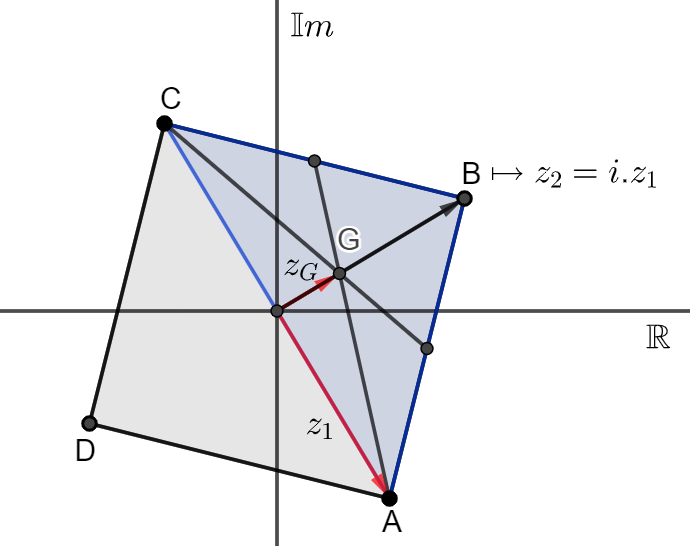
\includegraphics[scale=0.6]{ElonComplexosSol.png}
    \end{center}
     Por fim, como o triângulo $ABC$ é isósceles de base $AC$, segue que $OB$ é uma das medianas do triângulo. Sendo $G$ o braricentro do triângulo $ABC$, segue que $OG=\frac{1}{3}OB \Rightarrow z_G=\frac{1}{3}i.z_1$ (onde $z_G$ é o número complexo cujo afixo é o ponto $G$). Diante do exposto,
     $$z_G=\frac{1}{3} \cdot z_1=\frac{z_3}{3}\left(cos\frac{\pi}{2}+isen\frac{\pi}{2}\right).  $$

\noindent {\black \it Também recebemos uma solução correta de Yan Lima Machado}
\end{solution*}

\begin{problem*}
Qual o número de pares ordenados $(a,b)$ de inteiros positivos $a, b$ tais que as seguintes condições sejam simultaneamente satisfeitas?

%M

\begin{itemize}
    \item [$(i)$]  
    $a\mid 6000$;
    \item [$(ii)$] 
    $1\le b \le \frac{6000}{a}$;
     \item [$(ii)$]
     $\operatorname{mdc}(a, b,\frac{6000}{a}) = 1$.
\end{itemize}
\end{problem*}

\begin{solution*}
A função $f(n)$ que conta tais pares com $n$ no lugar de 6000 é multiplicativa, ou seja, $f(mn) = f(m)f(n)$ se $m,n$ são primos entre si.  Daí é fácil ver que $f(n) =n \cdot \prod_{p\mid n} (1 + \frac{1}{p})$ com $p$ primo.
\end{solution*}

\begin{problem*}
Seja $r(x)$ o polinômio que é o resto na divisão de $x^{2050}$ por $x^5 + x^2  +1$.  Quantos coeficientes ímpares possui $r(x)$?
\end{problem*}

%\begin{problem*}
%A sequência $a_n$ é definida por $a_1=\sqrt{2}$ e, para $n \geq 1$, $a_{n+1}=\sqrt{2+a_n}$. %Determine
%$$\lim_{n \to \infty} 4^n(2-a_n).$$
%\end{problem*}

%\begin{problem*}
%Uma função $F: \mathbb{R} \rightarrow \mathbb{R}$ é contínua e $F(x) \cdot F(F(x))=1$ para %todo $x$ real. Sabendo que 
%$F(1000)=999$, encontre $F(500)$.
%Leningrado 188 página 20
%\end{problem*}

\begin{solution*}
Vamos trabalhar no anel de polinômios 
$\mathbb{F}_2[x]$, em que $\mathbb{F}_2$ é 
o corpo dos inteiros módulo~2.  Neste anel, temos
$$  x^5 \equiv x^2 + 1 \pmod{x^5 + x^2 + 1}$$
implica que
$$  x^{10} \equiv (x^2 + 1)^2 \equiv x^4 + 1 \pmod{x^5 + x^2 + 1},$$
ou seja,
  \begin{align*}
  x^{20} &\equiv (x^4 + 1)^2 \\ 
  & \equiv x^8 + 1 \equiv x^3 (x^2+1) + 1 \\
  &\equiv x^2 + x^3 \pmod{x^5 + x^2 + 1}
  \end{align*}
e portanto, módulo $x^5 + x^2 + 1$,
\begin{eqnarray*}
    x^{30} &\equiv& (x^2 + x^3)\cdot (x^4 + 1) \\             &\equiv& x^7 + x^6 + x^3 + x^2\\
           &\equiv& x^2(x^2+1) + x(x^2+1) + x^3 + x^2\\ &\equiv& x^4 + x\\
    \implies x^{31} &\equiv& x^5 + x^2 \\
    &\equiv& 1
\end{eqnarray*}
(Uma maneira mais rápida de obter a última congruência seria perceber que $x^5 + x^2 + 1$ é irredutítvel em $\mathbb{F}_2[x]$, logo $\mathbb{F}_2[x]/(x^5 + x^2 + 1)$ é um corpo, extensão de $\mathbb{F}_2$ de grau~5, logo possui $2^5 = 32$ elementos e por Lagrange $a^{31} \equiv 1 \pmod{x^5 + x^2 + 1}$ se $a\not\equiv 0 \pmod{x^5 + x^2 + 1}$).
Por fim, $x^{2046} \equiv (x^{31})^{66} \equiv 1 \implies x^{2050} \equiv x^4$.  Assim, $r(x)$ é congruente a $x^4$ módulo $2$ e possui apenas 1 coeficiente ímpar.
\end{solution*}

\begin{problem*}
Considere $\Gamma$ o lugar geométrico dos pontos $P$ do plano cuja razão entre a distância de $P$ à origem e a distância entre $P$ e a reta $y=-1$ é constante e igual a $\frac{1}{2}$. Qual a maior distância entre dois pontos de $\Gamma$ ? 
	
\end{problem*}

\begin{solution*}

A descrição de tal lugar geométrico $\Gamma$ é de uma cônica com excentricidade $e = \frac{c}{a} = \frac{1}{2}$, ou seja, $\Gamma$ é uma elipse. Além disso, um dos focos dessa elipse é a origem e a reta $y = -1$ é uma diretriz. Assim, o eixo focal (sendo perpendicular à diretriz) é vertical, paralelo ao eixo $y$. De onde, o eixo focal é o próprio eixo $y$. Assim, a maior distância entre dois pontos de $\Gamma$ é exatamente o dobro do comprimento do semieixo maior, isto é, $2a$.

\vspace{0.3cm}

Para completar, sendo $A$ o vértice da elipse que 
está entre o foco $F_1 = (0,0)$ e a diretriz $r : y=-1$, 
temos $$1 + \frac{ d(A,r)}{d(A,F_1)} = \frac{d(A,F_1) + d(A,r)}{d(A,F_1)} = \frac{d(F_1,r)}{d(A,F_1)} = \frac{1}{d(A,F_1)}$$ 
e
$$a - c = d(A,F_1) = \frac{1}{1 + \frac{1}{e}} = \frac{1}{1+2} = \frac{1}{3}.$$ Também, $$\frac{c}{a} = \frac{1}{2} \ \ \Rightarrow \ \ c = \frac{a}{2}.$$ 
Então, $a - \frac{a}{2} = \frac{1}{3}$ e $a = \frac{2}{3}$. De onde, a máxima distância procurada é $2a = \frac{4}{3}$.

\noindent {\black \it Também recebemos uma solução correta de Yan Lima Machado}
\end{solution*}


\begin{problem*}
Seja $f : \mathbb{R} \rightarrow \mathbb{R}$ uma função ímpar e diferenciável satisfazendo:

\begin{itemize}
    \item $f(f(x)) = x$ para todo $x \in \mathbb{R}$;
    \item $f'(0) = -1$.
\end{itemize}

\noindent Mostre que $f(x) = -x$ para todo $x \in \mathbb{R}$.
	
\end{problem*}

\begin{solution*}

Como $f(f(x)) = x$ para todo $x \in \mathbb{R}$, 
então $f'(f(x)) \cdot f'(x) = 1$. De onde, $f'(x) \neq 0$, para todo $x \in \mathbb{R}$. 

\vspace{0.3cm}

Agora, se existisse $a$ tal que $f'(a) > 0$ e 
como $f'(0) = -1$, teríamos $$-1 = f'(0) < 0 < f'(a).$$ 
Então, pelo Teorema de Darboux 
(valor intermediário para a derivada), existiria $b$ entre $0$ e $a$ tal que $f'(b) = 0$, o que contraria o que acabamos de descobrir acima. Portanto, $f'(x) < 0$ para todo $x \in \mathbb{R}$, e $f$ é estritamente decrescente. 

\vspace{0.3cm}

Assim, se $f(x) > -x$ para algum $x$, então $x = f(f(x)) < f(-x) = -f(x)$, isto é, $f(x) < -x$ , sendo uma contradição. Analogamente, não pode ocorrer $f(x) < -x$. Portanto, $f(x) = -x$ para todo $x \in \mathbb{R}$. 

\end{solution*}


\begin{problem*}
Sejam $A, B \in M_n(\mathbb{R})$. Prove que $\mbox{rank}(A) + \mbox{rank}(B) \leq n$ se, e somente se, existe uma matriz invertível $X \in M_n(\mathbb{R})$ tal que $AXB = O_n$, onde $O_n$ é a matriz nula de ordem $n$.
	
\end{problem*}

\begin{solution*}
Queremos mostrar que $$\mbox{rank}(A) + \mbox{rank}(B) \leq n \ \ \ \ \Leftrightarrow \ \ \ \ \exists X \ \mbox{invertível} \ : \ AXB = O_n$$

$( \ \Leftarrow \ ) :$ Supondo a existência de uma matriz invertível $X$ satisfazendo $AXB = O_n$, pela desigualdade de Sylvester para o posto de matrizes, tem-se $$0 = \mbox{rank}(O_n) = \mbox{rank}(AXB) \geq \mbox{rank}(A) + \mbox{rank}(XB) - n $$ e $$\mbox{rank}(XB) \geq \mbox{rank}(B) + \mbox{rank}(X) - n $$ $$= \mbox{rank}(B) + n - n = \mbox{rank}(B).$$

Daí, $0 \geq \mbox{rank}(A) + \mbox{rank}(B) - n$, ou seja, $\mbox{rank}(A) + \mbox{rank}(B) \leq n$.



\vspace{0.3cm}
$( \ \Rightarrow \ ) :$ Estamos supondo agora que $\mbox{rank}(A) + \mbox{rank}(B) \leq n$. 
Existem matrizes inversíveis $X_A, Y_A, X_B$ e $Y_B$ 
tais que $$Y_A \cdot A \cdot X_A = \begin{bmatrix}
    I_{\mbox{rank}(A)} & \ \ 0 \\ 0 & \ \ O_{n - \mbox{rank}(A)}
\end{bmatrix}$$ e $$X_B \cdot B \cdot Y_B = \begin{bmatrix}
    O_{n - \mbox{rank}(B)} & \ \ 0 \\ 0 & \ \ I_{\mbox{rank}(B)} 
\end{bmatrix}$$ onde $I_{\mbox{rank}(A)}$ e $I_{\mbox{rank}(B)}$ são matrizes identidades de ordens $\mbox{rank}(A)$ e $\mbox{rank}(B)$, respectivamente. E $0$ ali representam matrizes nulas com as devidas ordens para preencherem as entradas restantes.
 Assim, multiplicando $Y_A \cdot A \cdot X_A$ e  
 $X_B \cdot B \cdot Y_B $, obtemos 
 $$\begin{bmatrix}
    I_{\mbox{rank}(A)} & \ \ 0 \\ 0 & \ \ O_{n - \mbox{rank}(A)}
\end{bmatrix} \cdot \begin{bmatrix}
    O_{n - \mbox{rank}(B)} & \ \ 0 \\ 0 & \ \ I_{\mbox{rank}(B)} 
\end{bmatrix} = O_n$$ 
essa última igualdade ocorre pois $n - \mbox{rank}(B) \geq \mbox{rank}(A)$  e $n - \mbox{rank}(A) \geq \mbox{rank}(B)$. 

\vspace{0.3cm}

Portanto, tomando $X = X_A \cdot X_B$ (que é invertível),
 obtemos $$AXB = Y_A^{-1} \cdot O_n \cdot Y_B^{-1} = O_n.$$
\end{solution*}


\section{Problemas de Matemática Elementar}

\begin{problem*}
Nas Olimpíadas de Pirajuba, existem $6$ competidores e $8$ dias de evento. Os três primeiros competidores de cada dia do evento recebem uma medalha, que pode ser de ouro, prata e bronze. Não existem empates e uma medalhade cada tipo é dada a apenas um atleta em cada dia do evento. Cada competidor recebe $5$ pontos por cada medalha de ouro, $3$ pontos por cada medalha de prata e $1$ ponto por cada medalha de bronze. Se Luciana, que é uma das competidoras, conseguiu um total de $27$ pontos no final do evento, qual o número máximo de medalhas de prata que ela pode ter recebido?
\end{problem*}

\begin{solution*}
Como são oito dias de evento, ela não pode ter ganho mais que $8$ medalhas de prata. Veja que essa quantidade não satisfaz o enunciado, pois $8 \cdot 3 = 24 < 27$. Assim, ela obteve menos de $8$ medalhas de prata. Vamos analisar os casos possíveis para determinar o número máximo de medalhas de prata que ela pode obter:
\begin{enumerate}[a)]
\item  Se ela tivesse obtido $7$ medalhas de prata, teria que fazer $27-3 \cdot 7 = 6$ pontos em um dia de evento, mas isso não é possível. 

\item Se ela tivesse obtido $6$ medalhas de prata, teria que fazer $27 - 3 \cdot 6 = 9$ pontos em dois dias de evento, mas isso não é possível pois $5+3<9<5+5$.

\item Se ela tivesse obtido $5$ medalhas de prata, teria que fazer $27 - 3 \cdot 5 = 12$ pontos em três dias de evento. Como $12> 3 \cdot 3$, pelo menos uma medalha de ouro, valendo $5$ pontos, teria que ser obtida. Por outro lado, não é possível combinar apenas duas parcelas de $1$, $3$ e $5$ para obter os $12-5 = 7$ pontos restantes. Consequentemente, ela não pode ter obtido $5$ medalhas de prata.
\end{enumerate}

\noindent Para mostrar que $4$ medalhas de prata é o máximo, basta exibirmos um exemplo. Após obter $3 \cdot 4 = 12$ pontos em $4$ dias com medalhas de prata, ela precisaria ter obtido  $27 - 3 \cdot 4 = 15$ pontos nos outros $4$ dias. Luciana pode obter essa pontuação com $3$ medalhas de ouro em $3$ dias e $1$ dia sem premiação.

\noindent {\black \it Também recebemos uma solução correta de Yan Lima Machado}
\end{solution*}

\begin{problem*}
Um encontro de britânicos e italianos em uma cafeteria reuniu 55 pessoas. Cada uma dessas pessoas pediu café ou chá. Sabemos que os britânicos sempre contam a verdade quando bebem chá e mentem quando bebem café. Já os italianos se comportam de modo oposto. Um repórter realizou uma rápida pesquisa e descobriu os seguintes fatos:
\begin{enumerate}
\item[1)] 44 pessoas responderam “sim” para a pergunta: “Você está bebendo café?”
\item[2)] 33 pessoas responderam “sim” para a pergunta: “Você é italiano?”
\item[3)] 22 pessoas concordaram com a afirmação: “Está chovendo lá fora”.
\end{enumerate}

Quantos britânicos na cafeteria estavam tomando chá?
\end{problem*}

\begin{solution*}
Qualquer pessoa que afirme estar bebendo café necessariamente precisa ser italiana. Portanto, existem $44$ italianos e $11$ britânicos.  Qualquer pessoa que afirme ser italiano tem que estar bebendo café. Portanto, havia 33 pessoas bebendo café. Seja $n$ o número de britânicos bebendo café. Então existiam $11-n$ britânicos bebendo chá, $33-n$ italianos bebendo café e $44-(33-n)=11+n$ italianos bebendo chá. Se não estava chovendo no lado de fora, então $n+(11+n)=22$, mas $n$ não é um inteiro nesse caso. Portanto, estava chovendo no exterior e $(11-n)+(33-n)=22$, consequentemente, $n=11$. Segue daí que $0$ britânicos estavam bebendo chá.
\end{solution*}

\begin{problem*}
Érica viajou para um país estrangeiro e sacou $\$800$ da moeda local em um banco. O caixa deu essa quantia usando notas de $\$20$, $\$50$ e $\$100$, usando pelo menos uma nota de cada tipo. De quantas maneiras diferentes ele pode ter feito esse pagamento para ela?
\end{problem*}

\begin{solution*}
 Se $x$, $y$ e $z$ são as quantias de notas de $\$20$, $\$50$ e $\$100$, respectivamente, portanto  $2x+5y+10z=80$. Como temos uma nota de cada tipo, podemos descontar uma $1$ unidade de cada uma das incógnitas anteriores e reduzir a equação para
$2a+5b+10c=63$.
Como $63$ é ímpar, precisamos que $b$ seja ímpar. Podemos analisar os casos. Quando $b=1$, 
$2a+10c=58$. Daí $10c=0,10,20,30,40$ ou $50$, ou seja, temos $6$ soluções. Quando $b=3$, $2a+10c=48$ e daí $10c=0,10,20,30$ ou $40$, ou seja, temos $5$ soluções. Continuando essa contagem, para $b=5$, $7$, $9$ e $11$, teremos  
$$6+5+4+3+2+1=21$$ soluções. 

\noindent {\black \it Também recebemos uma solução correta de Yan Lima Machado}
\end{solution*}


\begin{problem*}
Na malha a seguir, todos os quadradinhos possuem lados de mesma medida. Explique o porquê de os ângulos $\angle BAC$ e $\angle EDF$ possuírem a mesma medida. 
	
	\begin{center}	
		\begin{figure}[!h]
	\centering
	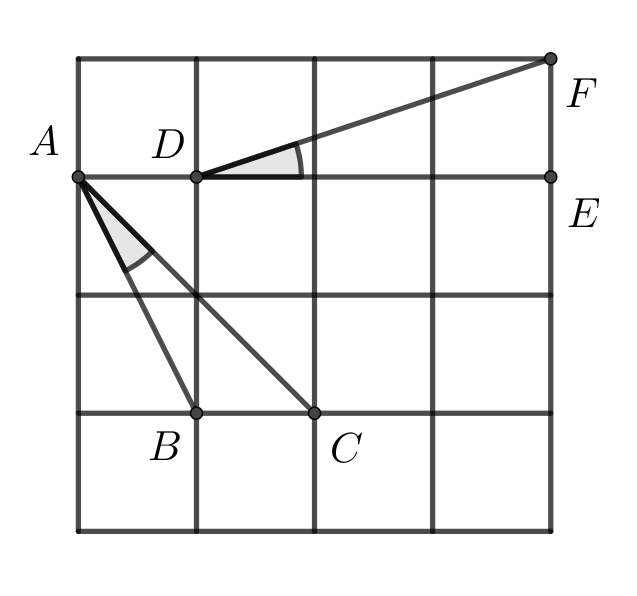
\includegraphics[width=0.3\linewidth]{2024S17.png}
\end{figure}
\end{center}	
\end{problem*}

\begin{solution*} {\black (Solução de Yan Lima Machado) Seja $BC=x$. Pelo Teorema de Pitágoras, tem-se que:
\begin{eqnarray*}
AB & = & \sqrt{5}x\\
AC & = & \sqrt{8}x \\
DF & = & \sqrt{10}x \\
\end{eqnarray*}

\noindent Ademais, considere $\angle BAC=\alpha$ e $\angle EDF=\beta$. Temos $\cos(\beta)=\frac{3x}{\sqrt{10}x}=\frac{3}{\sqrt{10}}$ e, pela Lei dos Cossenos no triângulo $ABC$, 
$x^{2}=8x^{2}+5x^{2}-4\sqrt{10}x^{2}\cos(\alpha)$, ou seja, $ \cos(\alpha)=\dfrac{12x^2}{4\sqrt{10}x^2} = \frac{3}{\sqrt{10}}$. Como $\alpha, \beta \in (0,\pi/2)$ e $\cos \alpha = \cos \beta$, segue que $\alpha = \beta$.}\\


\noindent Segunda Solução:
Note que $DH = HF$, pois ambos são diagonais de um retângulo $2 \times 1$ e, além disso, $\angle IHF = \angle IDH$.

	\begin{center}	
		\begin{figure}[!h]
	\centering
	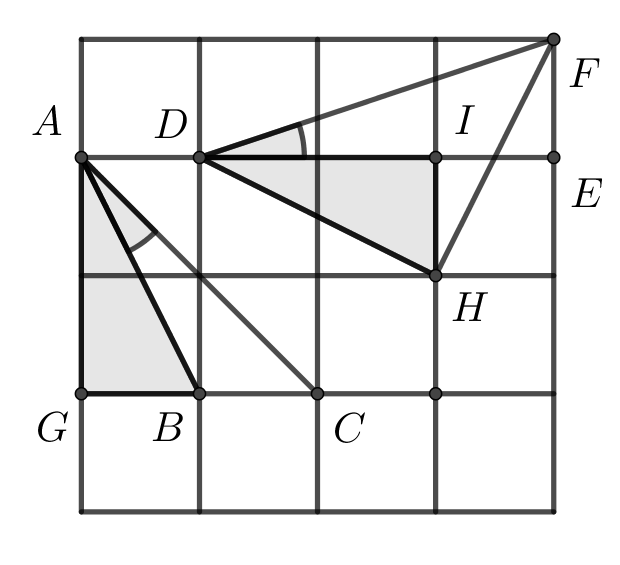
\includegraphics[width=0.3\linewidth]{2024S18.png}
\end{figure}
\end{center}	

\noindent Portanto, $$\angle DHF = \angle DHI + \angle IHF = \angle DHI + \angle HDI = 90^{\circ}.$$
Assim, $AGC$ e $DHF$ são ambos triângulos retângulos isósceles. Como os triângulos $AGB$ e $DHI$ são congruentes, segue que 
$$\angle BAC = 45^{\circ} - \angle BAG = 45^{\circ} - \angle HDI = \angle FDE.$$ 
\end{solution*}


\begin{problem*}
 Na figura a seguir, todos os triângulos são equiláteros e idênticos. Encontre a medida do ângulo $\angle ABC$.

\begin{center}



\tikzset{every picture/.style={line width=0.75pt}} %set default line width to 0.75pt        

\begin{tikzpicture}[x=0.75pt,y=0.75pt,yscale=-0.7,xscale=0.7]
%uncomment if require: \path (0,156); %set diagram left start at 0, and has height of 156

%Shape: Regular Polygon [id:dp42590613409471556] 
\draw   (101.6,127.59) -- (58.3,127.41) -- (80.11,90) -- cycle ;
%Shape: Regular Polygon [id:dp9891290054574801] 
\draw   (275.13,53.35) -- (231.83,53.16) -- (253.64,15.76) -- cycle ;
%Shape: Regular Polygon [id:dp432032311952501] 
\draw   (188.2,127.97) -- (144.9,127.78) -- (166.71,90.38) -- cycle ;
%Shape: Regular Polygon [id:dp965877053453182] 
\draw   (231.5,128.16) -- (188.2,127.97) -- (210.01,90.57) -- cycle ;
%Shape: Regular Polygon [id:dp60405412729036] 
\draw   (123.41,90.19) -- (80.11,90) -- (101.92,52.6) -- cycle ;
%Shape: Regular Polygon [id:dp38852321404456824] 
\draw   (166.71,90.38) -- (123.41,90.19) -- (145.22,52.78) -- cycle ;
%Shape: Regular Polygon [id:dp4093779740138518] 
\draw   (210.01,90.57) -- (166.71,90.38) -- (188.52,52.97) -- cycle ;
%Shape: Regular Polygon [id:dp2029637416434491] 
\draw   (80.11,90) -- (36.81,89.81) -- (58.62,52.41) -- cycle ;
%Shape: Regular Polygon [id:dp5343248854665051] 
\draw   (253.31,90.76) -- (210.01,90.57) -- (231.83,53.16) -- cycle ;
%Shape: Regular Polygon [id:dp6566631146501606] 
\draw   (101.92,52.6) -- (58.62,52.41) -- (80.44,15) -- cycle ;
%Shape: Regular Polygon [id:dp48167753179322537] 
\draw   (145.22,52.78) -- (101.92,52.6) -- (123.74,15.19) -- cycle ;
%Shape: Regular Polygon [id:dp6529080377153083] 
\draw   (188.52,52.97) -- (145.22,52.78) -- (167.04,15.38) -- cycle ;
%Shape: Regular Polygon [id:dp19072620498257065] 
\draw   (231.83,53.16) -- (188.52,52.97) -- (210.34,15.57) -- cycle ;
%Shape: Regular Polygon [id:dp5318721444025281] 
\draw   (144.9,127.78) -- (101.6,127.59) -- (123.41,90.19) -- cycle ;
%Shape: Regular Polygon [id:dp8872816823086344] 
\draw   (58.62,52.41) -- (15.32,52.22) -- (37.14,14.81) -- cycle ;
%Shape: Regular Polygon [id:dp3941974327848188] 
\draw   (37.27,14.73) -- (80.57,15.08) -- (58.62,52.41) -- cycle ;
%Shape: Regular Polygon [id:dp08330668174925715] 
\draw   (80.57,14.92) -- (123.87,15.27) -- (101.92,52.6) -- cycle ;
%Shape: Regular Polygon [id:dp1474450531110959] 
\draw   (123.87,15.27) -- (167.17,15.62) -- (145.22,52.94) -- cycle ;
%Shape: Regular Polygon [id:dp41036037730085884] 
\draw   (167.17,15.62) -- (210.47,15.97) -- (188.52,53.29) -- cycle ;
%Shape: Regular Polygon [id:dp6445074971855875] 
\draw   (210.47,15.97) -- (253.77,16.31) -- (231.82,53.64) -- cycle ;
%Shape: Regular Polygon [id:dp5435506141115087] 
\draw   (15.32,52.06) -- (58.62,52.41) -- (36.67,89.73) -- cycle ;
%Shape: Regular Polygon [id:dp045093785101125605] 
\draw   (36.81,89.81) -- (80.11,90.16) -- (58.16,127.48) -- cycle ;
%Shape: Regular Polygon [id:dp8659408226581283] 
\draw   (231.82,52.64) -- (275.12,52.99) -- (253.17,90.31) -- cycle ;
%Shape: Regular Polygon [id:dp00010682129482875169] 
\draw   (210.01,90.41) -- (253.31,90.76) -- (231.36,128.08) -- cycle ;
%Straight Lines [id:da8432136554916697] 
\draw [color={rgb, 255:red, 0; green, 0; blue, 0 }  ,draw opacity=1 ][line width=1.5]    (36.81,89.81) -- (231.36,128.08) ;
\draw [shift={(231.36,128.08)}, rotate = 11.13] [color={rgb, 255:red, 0; green, 0; blue, 0 }  ,draw opacity=1 ][fill={rgb, 255:red, 0; green, 0; blue, 0 }  ,fill opacity=1 ][line width=1.5]      (0, 0) circle [x radius= 4.36, y radius= 4.36]   ;
\draw [shift={(36.81,89.81)}, rotate = 11.13] [color={rgb, 255:red, 0; green, 0; blue, 0 }  ,draw opacity=1 ][fill={rgb, 255:red, 0; green, 0; blue, 0 }  ,fill opacity=1 ][line width=1.5]      (0, 0) circle [x radius= 4.36, y radius= 4.36]   ;
%Straight Lines [id:da36206940631647433] 
\draw [color={rgb, 255:red, 0; green, 0; blue, 0 }  ,draw opacity=1 ][line width=1.5]    (231.5,128.16) -- (253.77,16.31) ;
\draw [shift={(253.77,16.31)}, rotate = 281.26] [color={rgb, 255:red, 0; green, 0; blue, 0 }  ,draw opacity=1 ][fill={rgb, 255:red, 0; green, 0; blue, 0 }  ,fill opacity=1 ][line width=1.5]      (0, 0) circle [x radius= 4.36, y radius= 4.36]   ;
\draw [shift={(231.5,128.16)}, rotate = 281.26] [color={rgb, 255:red, 0; green, 0; blue, 0 }  ,draw opacity=1 ][fill={rgb, 255:red, 0; green, 0; blue, 0 }  ,fill opacity=1 ][line width=1.5]      (0, 0) circle [x radius= 4.36, y radius= 4.36]   ;

% Text Node
\draw (20,94.4) node [anchor=north west][inner sep=0.75pt]    {$A$};
% Text Node
\draw (233.5,131.56) node [anchor=north west][inner sep=0.75pt]    {$B$};
% Text Node
\draw (267,6.4) node [anchor=north west][inner sep=0.75pt]    {$C$};


\end{tikzpicture}

\end{center}
\end{problem*}

\newpage

\begin{solution*}{\black (Solução de Yan Lima Machado) Considere a medida dos lados dos triângulos igual a $x$ e sejam $D$, $E$, e $F$ os vértices marcados na figura a seguir.

\begin{center}
\tikzset{every picture/.style={line width=0.75pt}} %set default line width to 0.75pt        

\begin{tikzpicture}[x=0.75pt,y=0.75pt,yscale=-1,xscale=1]
%uncomment if require: \path (0,178); %set diagram left start at 0, and has height of 178

%Shape: Regular Polygon [id:dp08491158909105856] 
\draw   (97.6,134.59) -- (54.3,134.41) -- (76.11,97) -- cycle ;
%Shape: Regular Polygon [id:dp845026198083996] 
\draw   (271.13,60.35) -- (227.83,60.16) -- (249.64,22.76) -- cycle ;
%Shape: Regular Polygon [id:dp6612203545848362] 
\draw   (184.2,134.97) -- (140.9,134.78) -- (162.71,97.38) -- cycle ;
%Shape: Regular Polygon [id:dp34814278296626266] 
\draw   (227.5,135.16) -- (184.2,134.97) -- (206.01,97.57) -- cycle ;
%Shape: Regular Polygon [id:dp5173287672357627] 
\draw   (119.41,97.19) -- (76.11,97) -- (97.92,59.6) -- cycle ;
%Shape: Regular Polygon [id:dp7491117299043182] 
\draw   (162.71,97.38) -- (119.41,97.19) -- (141.22,59.78) -- cycle ;
%Shape: Regular Polygon [id:dp5122237351259774] 
\draw   (206.01,97.57) -- (162.71,97.38) -- (184.52,59.97) -- cycle ;
%Shape: Regular Polygon [id:dp09749066466418832] 
\draw   (76.11,97) -- (32.81,96.81) -- (54.62,59.41) -- cycle ;
%Shape: Regular Polygon [id:dp21751248950900304] 
\draw   (249.31,97.76) -- (206.01,97.57) -- (227.83,60.16) -- cycle ;
%Shape: Regular Polygon [id:dp10288151515995059] 
\draw   (97.92,59.6) -- (54.62,59.41) -- (76.44,22) -- cycle ;
%Shape: Regular Polygon [id:dp8059301140351733] 
\draw   (141.22,59.78) -- (97.92,59.6) -- (119.74,22.19) -- cycle ;
%Shape: Regular Polygon [id:dp9103722419978628] 
\draw   (184.52,59.97) -- (141.22,59.78) -- (163.04,22.38) -- cycle ;
%Shape: Regular Polygon [id:dp19200480233478057] 
\draw   (227.83,60.16) -- (184.52,59.97) -- (206.34,22.57) -- cycle ;
%Shape: Regular Polygon [id:dp9117702346343105] 
\draw   (140.9,134.78) -- (97.6,134.59) -- (119.41,97.19) -- cycle ;
%Shape: Regular Polygon [id:dp629969620445623] 
\draw   (54.62,59.41) -- (11.32,59.22) -- (33.14,21.81) -- cycle ;
%Shape: Regular Polygon [id:dp8766217694788297] 
\draw   (33.27,21.73) -- (76.57,22.08) -- (54.62,59.41) -- cycle ;
%Shape: Regular Polygon [id:dp03903379960580711] 
\draw   (76.57,21.92) -- (119.87,22.27) -- (97.92,59.6) -- cycle ;
%Shape: Regular Polygon [id:dp7986791883927549] 
\draw   (119.87,22.27) -- (163.17,22.62) -- (141.22,59.94) -- cycle ;
%Shape: Regular Polygon [id:dp007671303512082006] 
\draw   (163.17,22.62) -- (206.47,22.97) -- (184.52,60.29) -- cycle ;
%Shape: Regular Polygon [id:dp5281568599410649] 
\draw   (206.47,22.97) -- (249.77,23.31) -- (227.82,60.64) -- cycle ;
%Shape: Regular Polygon [id:dp0732252054478626] 
\draw   (11.32,59.06) -- (54.62,59.41) -- (32.67,96.73) -- cycle ;
%Shape: Regular Polygon [id:dp9095553706120761] 
\draw   (32.81,96.81) -- (76.11,97.16) -- (54.16,134.48) -- cycle ;
%Shape: Regular Polygon [id:dp3502064583274721] 
\draw   (227.82,59.64) -- (271.12,59.99) -- (249.17,97.31) -- cycle ;
%Shape: Regular Polygon [id:dp8993526029788339] 
\draw   (206.01,97.41) -- (249.31,97.76) -- (227.36,135.08) -- cycle ;
%Straight Lines [id:da7916805163435271] 
\draw [color={rgb, 255:red, 0; green, 0; blue, 0 }  ,draw opacity=1 ][line width=1.5]    (32.81,96.81) -- (227.36,135.08) ;
\draw [shift={(227.36,135.08)}, rotate = 11.13] [color={rgb, 255:red, 0; green, 0; blue, 0 }  ,draw opacity=1 ][fill={rgb, 255:red, 0; green, 0; blue, 0 }  ,fill opacity=1 ][line width=1.5]      (0, 0) circle [x radius= 4.36, y radius= 4.36]   ;
\draw [shift={(32.81,96.81)}, rotate = 11.13] [color={rgb, 255:red, 0; green, 0; blue, 0 }  ,draw opacity=1 ][fill={rgb, 255:red, 0; green, 0; blue, 0 }  ,fill opacity=1 ][line width=1.5]      (0, 0) circle [x radius= 4.36, y radius= 4.36]   ;
%Straight Lines [id:da33441801912221814] 
\draw [color={rgb, 255:red, 0; green, 0; blue, 0 }  ,draw opacity=1 ][line width=1.5]    (227.5,135.16) -- (249.77,23.31) ;
\draw [shift={(249.77,23.31)}, rotate = 281.26] [color={rgb, 255:red, 0; green, 0; blue, 0 }  ,draw opacity=1 ][fill={rgb, 255:red, 0; green, 0; blue, 0 }  ,fill opacity=1 ][line width=1.5]      (0, 0) circle [x radius= 4.36, y radius= 4.36]   ;
\draw [shift={(227.5,135.16)}, rotate = 281.26] [color={rgb, 255:red, 0; green, 0; blue, 0 }  ,draw opacity=1 ][fill={rgb, 255:red, 0; green, 0; blue, 0 }  ,fill opacity=1 ][line width=1.5]      (0, 0) circle [x radius= 4.36, y radius= 4.36]   ;
%Straight Lines [id:da5596414931824846] 
\draw [color={rgb, 255:red, 0; green, 0; blue, 0 }  ,draw opacity=1 ][line width=1.5]    (33.14,21.81) -- (249.77,23.31) ;
\draw [shift={(249.77,23.31)}, rotate = 0.4] [color={rgb, 255:red, 0; green, 0; blue, 0 }  ,draw opacity=1 ][fill={rgb, 255:red, 0; green, 0; blue, 0 }  ,fill opacity=1 ][line width=1.5]      (0, 0) circle [x radius= 4.36, y radius= 4.36]   ;
\draw [shift={(33.14,21.81)}, rotate = 0.4] [color={rgb, 255:red, 0; green, 0; blue, 0 }  ,draw opacity=1 ][fill={rgb, 255:red, 0; green, 0; blue, 0 }  ,fill opacity=1 ][line width=1.5]      (0, 0) circle [x radius= 4.36, y radius= 4.36]   ;
%Straight Lines [id:da7981179871743741] 
\draw [color={rgb, 255:red, 0; green, 0; blue, 0 }  ,draw opacity=1 ][line width=1.5]    (33.14,21.81) -- (32.81,96.81) ;
\draw [shift={(32.81,96.81)}, rotate = 90.25] [color={rgb, 255:red, 0; green, 0; blue, 0 }  ,draw opacity=1 ][fill={rgb, 255:red, 0; green, 0; blue, 0 }  ,fill opacity=1 ][line width=1.5]      (0, 0) circle [x radius= 4.36, y radius= 4.36]   ;
\draw [shift={(33.14,21.81)}, rotate = 90.25] [color={rgb, 255:red, 0; green, 0; blue, 0 }  ,draw opacity=1 ][fill={rgb, 255:red, 0; green, 0; blue, 0 }  ,fill opacity=1 ][line width=1.5]      (0, 0) circle [x radius= 4.36, y radius= 4.36]   ;
%Straight Lines [id:da7555491145562852] 
\draw [color={rgb, 255:red, 0; green, 0; blue, 0 }  ,draw opacity=1 ][line width=1.5]    (32.81,96.81) -- (249.77,23.31) ;
\draw [shift={(249.77,23.31)}, rotate = 341.29] [color={rgb, 255:red, 0; green, 0; blue, 0 }  ,draw opacity=1 ][fill={rgb, 255:red, 0; green, 0; blue, 0 }  ,fill opacity=1 ][line width=1.5]      (0, 0) circle [x radius= 4.36, y radius= 4.36]   ;
\draw [shift={(32.81,96.81)}, rotate = 341.29] [color={rgb, 255:red, 0; green, 0; blue, 0 }  ,draw opacity=1 ][fill={rgb, 255:red, 0; green, 0; blue, 0 }  ,fill opacity=1 ][line width=1.5]      (0, 0) circle [x radius= 4.36, y radius= 4.36]   ;
%Straight Lines [id:da6996316444813242] 
\draw [color={rgb, 255:red, 0; green, 0; blue, 0 }  ,draw opacity=1 ][line width=1.5]    (271.13,60.35) -- (227.36,135.08) ;
\draw [shift={(227.36,135.08)}, rotate = 120.35] [color={rgb, 255:red, 0; green, 0; blue, 0 }  ,draw opacity=1 ][fill={rgb, 255:red, 0; green, 0; blue, 0 }  ,fill opacity=1 ][line width=1.5]      (0, 0) circle [x radius= 4.36, y radius= 4.36]   ;
\draw [shift={(271.13,60.35)}, rotate = 120.35] [color={rgb, 255:red, 0; green, 0; blue, 0 }  ,draw opacity=1 ][fill={rgb, 255:red, 0; green, 0; blue, 0 }  ,fill opacity=1 ][line width=1.5]      (0, 0) circle [x radius= 4.36, y radius= 4.36]   ;
%Straight Lines [id:da3429481070796504] 
\draw [color={rgb, 255:red, 0; green, 0; blue, 0 }  ,draw opacity=1 ][line width=1.5]    (249.77,23.31) -- (271.13,60.35) ;
\draw [shift={(271.13,60.35)}, rotate = 60.04] [color={rgb, 255:red, 0; green, 0; blue, 0 }  ,draw opacity=1 ][fill={rgb, 255:red, 0; green, 0; blue, 0 }  ,fill opacity=1 ][line width=1.5]      (0, 0) circle [x radius= 4.36, y radius= 4.36]   ;
\draw [shift={(249.77,23.31)}, rotate = 60.04] [color={rgb, 255:red, 0; green, 0; blue, 0 }  ,draw opacity=1 ][fill={rgb, 255:red, 0; green, 0; blue, 0 }  ,fill opacity=1 ][line width=1.5]      (0, 0) circle [x radius= 4.36, y radius= 4.36]   ;
%Straight Lines [id:da005211606369438071] 
\draw [color={rgb, 255:red, 0; green, 0; blue, 0 }  ,draw opacity=1 ][line width=1.5]    (54.3,134.41) -- (227.5,135.16) ;
\draw [shift={(227.5,135.16)}, rotate = 0.25] [color={rgb, 255:red, 0; green, 0; blue, 0 }  ,draw opacity=1 ][fill={rgb, 255:red, 0; green, 0; blue, 0 }  ,fill opacity=1 ][line width=1.5]      (0, 0) circle [x radius= 4.36, y radius= 4.36]   ;
\draw [shift={(54.3,134.41)}, rotate = 0.25] [color={rgb, 255:red, 0; green, 0; blue, 0 }  ,draw opacity=1 ][fill={rgb, 255:red, 0; green, 0; blue, 0 }  ,fill opacity=1 ][line width=1.5]      (0, 0) circle [x radius= 4.36, y radius= 4.36]   ;
%Straight Lines [id:da03568660030716564] 
\draw [color={rgb, 255:red, 0; green, 0; blue, 0 }  ,draw opacity=1 ][line width=1.5]    (32.67,96.73) -- (54.16,134.48) ;
\draw [shift={(54.16,134.48)}, rotate = 60.36] [color={rgb, 255:red, 0; green, 0; blue, 0 }  ,draw opacity=1 ][fill={rgb, 255:red, 0; green, 0; blue, 0 }  ,fill opacity=1 ][line width=1.5]      (0, 0) circle [x radius= 4.36, y radius= 4.36]   ;
\draw [shift={(32.67,96.73)}, rotate = 60.36] [color={rgb, 255:red, 0; green, 0; blue, 0 }  ,draw opacity=1 ][fill={rgb, 255:red, 0; green, 0; blue, 0 }  ,fill opacity=1 ][line width=1.5]      (0, 0) circle [x radius= 4.36, y radius= 4.36]   ;

% Text Node
\draw (16,101.4) node [anchor=north west][inner sep=0.75pt]    {$A$};
% Text Node
\draw (229.5,138.56) node [anchor=north west][inner sep=0.75pt]    {$B$};
% Text Node
\draw (263,13.4) node [anchor=north west][inner sep=0.75pt]    {$C$};
% Text Node
\draw (14,3.4) node [anchor=north west][inner sep=0.75pt]    {$E$};
% Text Node
\draw (70,138.4) node [anchor=north west][inner sep=0.75pt]    {$x$};
% Text Node
\draw (273.13,63.75) node [anchor=north west][inner sep=0.75pt]    {$F$};
% Text Node
\draw (35,138.4) node [anchor=north west][inner sep=0.75pt]    {$D$};


\end{tikzpicture}


\end{center}

\noindent Como o triângulo $AEC$ é retângulo em $E$, pois $AE$ é mediatriz de um dos segmentos da malha, temos pelo Teorema de Pitágoras:
\begin{eqnarray*}
 AC^2 & = & AE^2 + EC^2 \\
      & = & 3x^2+ 25x^2 \\
      & = & 28x^2.
\end{eqnarray*}
Pela Lei dos Cossenos nos triângulos $ADB$ e $BCF$, temos 
\begin{eqnarray*}
 AB^2 & = & AD^2-2AD \cdot DB \cdot \cos 120^{\circ} + DB^2 \\
      & = & x^{2}-2\cdot4x^{2}(\frac{-1}{2}) +16x^{2}\\
      & = & 21x^2
\end{eqnarray*}
e 
\begin{eqnarray*}
BC^2 & = & CF^2-2CF \cdot FB \cdot \cos 120^{\circ} + FB^2 \\
      & = & x^{2}-2\cdot2x^{2}(\frac{-1}{2})+4x^{2}\\
      & = & 7x^2.
\end{eqnarray*}
Como $AC^2=AB^2+BC^2$, pela recíproca do Teorema de Pitágoras, temos que $\angle ABC=90^{\circ}$}\\

\noindent Segunda Solução:
\noindent Continue o ladrilhamento com triângulos equiláteros como na figura anterior. 
\begin{center}


\tikzset{every picture/.style={line width=0.75pt}} %set default line width to 0.75pt        

\begin{tikzpicture}[x=0.75pt,y=0.75pt,yscale=-0.7,xscale=0.7]
%uncomment if require: \path (0,271); %set diagram left start at 0, and has height of 271

%Shape: Regular Polygon [id:dp21895116602857045] 
\draw   (106.6,134.59) -- (63.3,134.41) -- (85.11,97) -- cycle ;
%Shape: Regular Polygon [id:dp9344167892728236] 
\draw   (280.13,60.35) -- (236.83,60.16) -- (258.64,22.76) -- cycle ;
%Shape: Regular Polygon [id:dp2154756689199716] 
\draw   (193.2,134.97) -- (149.9,134.78) -- (171.71,97.38) -- cycle ;
%Shape: Regular Polygon [id:dp1371356183594522] 
\draw   (236.5,135.16) -- (193.2,134.97) -- (215.01,97.57) -- cycle ;
%Shape: Regular Polygon [id:dp822877161776802] 
\draw   (128.41,97.19) -- (85.11,97) -- (106.92,59.6) -- cycle ;
%Shape: Regular Polygon [id:dp7539861820744734] 
\draw   (171.71,97.38) -- (128.41,97.19) -- (150.22,59.78) -- cycle ;
%Shape: Regular Polygon [id:dp993965741313323] 
\draw   (215.01,97.57) -- (171.71,97.38) -- (193.52,59.97) -- cycle ;
%Shape: Regular Polygon [id:dp7547378798208753] 
\draw   (85.11,97) -- (41.81,96.81) -- (63.62,59.41) -- cycle ;
%Shape: Regular Polygon [id:dp7892094855708801] 
\draw   (258.31,97.76) -- (215.01,97.57) -- (236.83,60.16) -- cycle ;
%Shape: Regular Polygon [id:dp8267588135338169] 
\draw   (106.92,59.6) -- (63.62,59.41) -- (85.44,22) -- cycle ;
%Shape: Regular Polygon [id:dp5572222642215952] 
\draw   (150.22,59.78) -- (106.92,59.6) -- (128.74,22.19) -- cycle ;
%Shape: Regular Polygon [id:dp32610310927515207] 
\draw   (193.52,59.97) -- (150.22,59.78) -- (172.04,22.38) -- cycle ;
%Shape: Regular Polygon [id:dp431311829675193] 
\draw   (236.83,60.16) -- (193.52,59.97) -- (215.34,22.57) -- cycle ;
%Shape: Regular Polygon [id:dp6987273806247992] 
\draw   (149.9,134.78) -- (106.6,134.59) -- (128.41,97.19) -- cycle ;
%Shape: Regular Polygon [id:dp12734371681682277] 
\draw   (63.62,59.41) -- (20.32,59.22) -- (42.14,21.81) -- cycle ;
%Shape: Regular Polygon [id:dp5881952402010149] 
\draw   (42.27,21.73) -- (85.57,22.08) -- (63.62,59.41) -- cycle ;
%Shape: Regular Polygon [id:dp9681411664142879] 
\draw   (85.57,21.92) -- (128.87,22.27) -- (106.92,59.6) -- cycle ;
%Shape: Regular Polygon [id:dp1468301076776274] 
\draw   (128.87,22.27) -- (172.17,22.62) -- (150.22,59.94) -- cycle ;
%Shape: Regular Polygon [id:dp26393420038207005] 
\draw   (172.17,22.62) -- (215.47,22.97) -- (193.52,60.29) -- cycle ;
%Shape: Regular Polygon [id:dp4485418032670895] 
\draw   (215.47,22.97) -- (258.77,23.31) -- (236.82,60.64) -- cycle ;
%Shape: Regular Polygon [id:dp7758270533866701] 
\draw   (20.32,59.06) -- (63.62,59.41) -- (41.67,96.73) -- cycle ;
%Shape: Regular Polygon [id:dp43937382473630693] 
\draw   (41.81,96.81) -- (85.11,97.16) -- (63.16,134.48) -- cycle ;
%Shape: Regular Polygon [id:dp6400672252246518] 
\draw   (236.82,59.64) -- (280.12,59.99) -- (258.17,97.31) -- cycle ;
%Shape: Regular Polygon [id:dp9896598166219387] 
\draw   (215.01,97.41) -- (258.31,97.76) -- (236.36,135.08) -- cycle ;
%Straight Lines [id:da2769868407310998] 
\draw [color={rgb, 255:red, 0; green, 0; blue, 0 }  ,draw opacity=1 ][line width=1.5]    (41.81,96.81) -- (236.36,135.08) ;
\draw [shift={(236.36,135.08)}, rotate = 11.13] [color={rgb, 255:red, 0; green, 0; blue, 0 }  ,draw opacity=1 ][fill={rgb, 255:red, 0; green, 0; blue, 0 }  ,fill opacity=1 ][line width=1.5]      (0, 0) circle [x radius= 4.36, y radius= 4.36]   ;
\draw [shift={(41.81,96.81)}, rotate = 11.13] [color={rgb, 255:red, 0; green, 0; blue, 0 }  ,draw opacity=1 ][fill={rgb, 255:red, 0; green, 0; blue, 0 }  ,fill opacity=1 ][line width=1.5]      (0, 0) circle [x radius= 4.36, y radius= 4.36]   ;
%Straight Lines [id:da5344142794543654] 
\draw [color={rgb, 255:red, 0; green, 0; blue, 0 }  ,draw opacity=1 ][line width=1.5]    (236.5,135.16) -- (258.77,23.31) ;
\draw [shift={(258.77,23.31)}, rotate = 281.26] [color={rgb, 255:red, 0; green, 0; blue, 0 }  ,draw opacity=1 ][fill={rgb, 255:red, 0; green, 0; blue, 0 }  ,fill opacity=1 ][line width=1.5]      (0, 0) circle [x radius= 4.36, y radius= 4.36]   ;
\draw [shift={(236.5,135.16)}, rotate = 281.26] [color={rgb, 255:red, 0; green, 0; blue, 0 }  ,draw opacity=1 ][fill={rgb, 255:red, 0; green, 0; blue, 0 }  ,fill opacity=1 ][line width=1.5]      (0, 0) circle [x radius= 4.36, y radius= 4.36]   ;
%Shape: Regular Polygon [id:dp20264494221905938] 
\draw   (128.08,172.19) -- (84.78,172) -- (106.6,134.59) -- cycle ;
%Shape: Regular Polygon [id:dp5632146742994568] 
\draw   (171.38,172.38) -- (128.08,172.19) -- (149.9,134.78) -- cycle ;
%Shape: Regular Polygon [id:dp05920579218617894] 
\draw   (214.68,172.57) -- (171.38,172.38) -- (193.2,134.97) -- cycle ;
%Shape: Regular Polygon [id:dp3571297279201069] 
\draw   (149.57,209.78) -- (106.27,209.59) -- (128.08,172.19) -- cycle ;
%Shape: Regular Polygon [id:dp24542717031431605] 
\draw   (192.87,209.97) -- (149.57,209.78) -- (171.38,172.38) -- cycle ;
%Shape: Regular Polygon [id:dp5037394344429463] 
\draw   (63.3,134.25) -- (106.6,134.59) -- (84.64,171.92) -- cycle ;
%Shape: Regular Polygon [id:dp06987292167387515] 
\draw   (84.78,171.84) -- (128.08,172.19) -- (106.13,209.51) -- cycle ;
%Shape: Regular Polygon [id:dp08605462761628246] 
\draw   (193.06,134.73) -- (236.36,135.08) -- (214.41,172.41) -- cycle ;
%Shape: Regular Polygon [id:dp6708900128052145] 
\draw   (171.11,172.06) -- (214.41,172.41) -- (192.46,209.73) -- cycle ;
%Shape: Regular Polygon [id:dp7512356617612356] 
\draw   (257.71,172.59) -- (214.41,172.41) -- (236.22,135) -- cycle ;
%Shape: Regular Polygon [id:dp45313447591496614] 
\draw   (236.17,210.16) -- (192.87,209.97) -- (214.68,172.57) -- cycle ;
%Shape: Regular Polygon [id:dp06331347199998727] 
\draw   (171.06,247.38) -- (127.76,247.19) -- (149.57,209.78) -- cycle ;
%Shape: Regular Polygon [id:dp32564188279914397] 
\draw   (213.95,247.33) -- (170.65,247.14) -- (192.46,209.73) -- cycle ;
%Shape: Regular Polygon [id:dp09307541069700376] 
\draw   (279.8,135.35) -- (236.5,135.16) -- (258.31,97.76) -- cycle ;
%Shape: Regular Polygon [id:dp9313717470611277] 
\draw   (301.61,97.94) -- (258.31,97.76) -- (280.13,60.35) -- cycle ;
%Shape: Regular Polygon [id:dp34903567705628913] 
\draw   (258.31,97.76) -- (301.61,98.1) -- (279.66,135.43) -- cycle ;
%Shape: Regular Polygon [id:dp9997115407644052] 
\draw   (236.22,135) -- (279.52,135.35) -- (257.57,172.67) -- cycle ;
%Shape: Regular Polygon [id:dp24458564121438064] 
\draw   (214.68,172.57) -- (257.98,172.91) -- (236.03,210.24) -- cycle ;
%Shape: Regular Polygon [id:dp7755927452502124] 
\draw   (192.87,209.81) -- (236.17,210.16) -- (214.22,247.49) -- cycle ;
%Shape: Regular Polygon [id:dp5920889052275203] 
\draw   (106.13,209.51) -- (149.43,209.86) -- (127.48,247.19) -- cycle ;
%Straight Lines [id:da35951841880861624] 
\draw [color={rgb, 255:red, 0; green, 0; blue, 0 }  ,draw opacity=1 ][line width=1.5]    (213.95,246.85) -- (236.22,135) ;
\draw [shift={(236.22,135)}, rotate = 281.26] [color={rgb, 255:red, 0; green, 0; blue, 0 }  ,draw opacity=1 ][fill={rgb, 255:red, 0; green, 0; blue, 0 }  ,fill opacity=1 ][line width=1.5]      (0, 0) circle [x radius= 4.36, y radius= 4.36]   ;
\draw [shift={(213.95,246.85)}, rotate = 281.26] [color={rgb, 255:red, 0; green, 0; blue, 0 }  ,draw opacity=1 ][fill={rgb, 255:red, 0; green, 0; blue, 0 }  ,fill opacity=1 ][line width=1.5]      (0, 0) circle [x radius= 4.36, y radius= 4.36]   ;
%Straight Lines [id:da8232510043669715] 
\draw [fill={rgb, 255:red, 155; green, 155; blue, 155 }  ,fill opacity=0.4 ]   (41.81,96.81) -- (128.41,97.19) -- (213.95,247.33) -- (127.48,247.19) -- (41.81,96.81) ;
%Straight Lines [id:da20264377326852567] 
\draw [fill={rgb, 255:red, 155; green, 155; blue, 155 }  ,fill opacity=0.4 ]   (41.67,96.73) -- (85.57,22.08) -- (258.77,23.31) -- (215.01,97.57) -- (41.81,96.81) ;
%Straight Lines [id:da08380061494586577] 
\draw [line width=1.5]  [dash pattern={on 5.63pt off 4.5pt}]  (41.81,96.81) -- (258.77,23.31) ;
%Straight Lines [id:da5125648211206376] 
\draw [line width=1.5]  [dash pattern={on 5.63pt off 4.5pt}]  (41.81,96.81) -- (214.22,247.49) ;

% Text Node
\draw (25,101.4) node [anchor=north west][inner sep=0.75pt]    {$A$};
% Text Node
\draw (238.5,138.56) node [anchor=north west][inner sep=0.75pt]    {$B$};
% Text Node
\draw (272,13.4) node [anchor=north west][inner sep=0.75pt]    {$C$};
% Text Node
\draw (216.22,250.89) node [anchor=north west][inner sep=0.75pt]    {$D$};


\end{tikzpicture}

\end{center}	

\noindent  Note que o segmento $CB$ é a diagonal de um paralelogramo formado por $4$ triângulos do reticulado e, por simetria, o seu prolongamento irá encontrar o vértice $D$ de outro paralelogramo também formado por $4$ triângulos do reticulado. Tanto $AD$ quanto $AC$ são diagonais de paralelogramos congruentes, que estão pintados de cinza no desenho, portanto, $AC = AD$. Assim, como $B$ é o ponto médio de $CD$, o segmento $AB$ é uma altura do triângulo isósceles $ACD$ e daí $\angle ABC = 90^{\circ}$. 
\end{solution*}


\begin{problem*}
Prove que $$\frac{1}{15} < \frac{1}{2}\cdot \frac{3}{4} \cdot \frac{5}{6} \cdots \frac{99}{100} < \frac{1}{12}$$
	
\end{problem*}

\begin{solution*}
Se $$K = \frac{1}{2}\cdot \frac{3}{4} \cdot \frac{5}{6} \cdots \frac{99}{100},$$ temos
$$K  > \frac{1}{2}\cdot \frac{2}{3} \cdot \frac{4}{5} \cdots \frac{98}{99}.$$
Portanto, multiplicando a igualdade anterior por essa última desigualdade, obtemos:
$$K^2 > \dfrac{1}{200} > \dfrac{1}{225},$$
ou seja, 
$$K > \dfrac{1}{15}.$$

Agora, para mostrar a outra desigualdade do problema, temos 

\begin{eqnarray*}
K & =&  \frac{1}{2} \cdot \frac{3}{4} \cdot \frac{5}{6} \cdot \frac{7}{8}\cdots \frac{97}{98}\cdot \frac{99}{100} \\ 
&<& \frac{1}{2} \cdot \frac{3}{4} \cdot \frac{5}{6} \cdot \left(\frac{8}{9} \cdots \frac{98}{99} \cdot  \frac{100}{101} \right)\cdot \frac{2}{3} \cdot \frac{4}{5} \cdot \frac{6}{7} \cdot \frac{3}{2} \cdot \frac{5}{4} \cdot \frac{7}{6} \\ &=& \frac{1}{2} \cdot \frac{3}{4} \cdot \frac{5}{6} \cdot \frac{3}{2} \cdot \frac{5}{4} \cdot \frac{7}{6} \cdot \left(\frac{2}{3} \cdot \frac{4}{5} \cdot \frac{6}{7}  \cdot \frac{8}{9} \cdots \frac{98}{99} \cdot  \frac{100}{101} \right)
\end{eqnarray*}
O último membro pode ser reescrito como
$$ \frac{1}{2} \cdot \frac{3}{4} \cdot \frac{5}{6} \cdot \frac{3}{2} \cdot \frac{5}{4} \cdot \frac{7}{6} \cdot \frac{1}{101K} = \frac{175}{16 \cdot 16 \cdot 101K}$$ 
Daí,
$$K^2 < \frac{175}{16 \cdot 1616} < \frac{175}{16 \cdot 1575} = \frac{175}{16 \cdot 9 \cdot 175} = \frac{1}{144} = \frac{1}{12^2}$$ e, portanto, $K < \frac{1}{12}$. Logo, $$\frac{1}{15} < K < \frac{1}{12}.$$
\end{solution*}


\begin{problem*}
Avalie a soma simplificando ao máximo sua expressão $$\frac{2}{0! + 1! + 2!} + \frac{3}{1! + 2! + 3!} + \cdots + \frac{2024}{2022! + 2023! + 2024!}. $$
	
\end{problem*}

\begin{solution*}
Queremos simplicar ao máximo a expressão da soma $$\frac{2}{0! + 1! + 2!} + \frac{3}{1! + 2! + 3!} + \cdots + \frac{2024}{2022! + 2023! + 2024!} .$$

Veja que $$\frac{k}{(k-2)! + (k-1)! + k!} = \frac{k}{(k-2)! \cdot [1 + (k-1) + (k-1)k]} $$ $$= \frac{k}{(k-2)! \cdot (k + k^2 - k)} = \frac{k}{(k-2)!k^2} = \frac{k-1}{(k-2)!(k-1)k} $$ $$= \frac{k-1}{k!} = \frac{1}{(k-1)!} - \frac{1}{k!}.$$

Daí, $$\sum_{k=2}^{2024} \ \ \frac{k}{(k-2)! + (k-1)! + k!} = \sum_{k=2}^{2024} \ \ \frac{1}{(k-1)!} - \frac{1}{k!}$$ é uma soma telescópica. Com isso, $$\frac{2}{0! + 1! + 2!} + \frac{3}{1! + 2! + 3!} + \cdots + \frac{2024}{2022! + 2023! + 2024!} $$ $$= \left( 1 - \frac{1}{2!} \right) + \left( \frac{1}{2!} - \frac{1}{3!} \right) + \cdots + \left( \frac{1}{2023!} - \frac{1}{2024!} \right) = 1 - \frac{1}{2024!}.$$

{\black \it Também recebemos uma solução correta de Yan Lima Machado}
\end{solution*}
%%%%%%%%%%%%%%%%%%%%%%%%%%%%%%%%%%%%%%%%%%%%%%%%%%%%%%%%%%%%%%%%%%%%%%%%%%%%%%%%%%%%%%%%%%%%%%%%%%%%%%%%%%%%%%%%%%%%%%%%%%%%%%%%%%%%%%%%%%%%%%%%%%%%%%%%%%%%%%%%%%%%%%%%%%%%%%%%%%%%%%%%%%%%%%%%%%%%%%%%%%%%%%%%%%%%%%%%%%%%

\section{Novos Problemas}

\section{Problemas Universitários}

\begin{problem*}
Sejam $A_1, A_2, \ldots, A_{n+1}$ subconjuntos não vazios de $\{1,2,\ldots, n\}$. Prove que existem conjuntos de índices disjuntos e não vazios 
$I,J \subset \{1,2,\ldots, n+1\}$ tais que $$\displaystyle \bigcup_{k \in I} A_k = \bigcup_{k \in J} A_k.$$
\end{problem*}

\begin{problem*}
Dizemos que um grupo $G=(G,\ast)$ tem raiz se existe um grupo $H=(H,\cdot)$ de tal sorte que $G$ é isomorfo a $H \times H$. Mostre que o grupo $(\mathbb{R}, +)$ não possui raiz.

\noindent Dica: Tente ver a possível raíz como um subespaço vetorial de $\mathbb{R}$ sobre $\mathbb{Q}$. Como construir uma base para esse espaço vetorial?	

\end{problem*}

\begin{problem*}
Seja $G$ um conjunto finito de matrizes $n \times n$ de coeficientes reais $\{M_i\}$, $1 \leq i \leq r$, que forma um grupo sobre a multiplicação matricial. Suponha que $\sum_{i=1}^{r} tr(M_i)=0$, onde $tr(A)$ denota o traço da matriz $A$. Prove que $\sum_{i=1}^r M_i$ é a matriz nula.     
\end{problem*}

\begin{problem*}
Seja $f(x)=a_1\sin x+a_2 \sin 2x+\ldots +a_n \sin nx$, onde $a_1,a_2, \ldots, a_n$ são números reais e $n$ é um inteiro positivo. Dado que $|f(x)|\leq |\sin x|$ para todo o número real $x$, prove que $|a_1+2a_2+\ldots+na_n| \leq 1$.
% 108 larson    
\end{problem*}

\begin{problem*}
Calcule a integral
$$\displaystyle \int_{0}^{\pi/2} \dfrac{\sin^{25}x}{\cos^{25}x+\sin^{25}x}dx.$$    
\end{problem*}

\section{Problemas de Matemática Elementar}

\begin{problem*}
A figura a seguir consiste de $5$ quadrados iguais colocados no interior de um retângulo $8 cm \times 7 cm$. Qual a medida do lado desses quadrados?


\begin{center}
%\includegraphics[scale=1]{2025S5.png} 



\tikzset{every picture/.style={line width=0.75pt}} %set default line width to 0.75pt        

\begin{tikzpicture}[x=0.75pt,y=0.75pt,yscale=-0.8,xscale=0.8]
%uncomment if require: \path (0,229); %set diagram left start at 0, and has height of 229

%Shape: Square [id:dp8310591847333366] 
\draw   (81.04,143.73) -- (126.27,165.04) -- (104.96,210.27) -- (59.73,188.96) -- cycle ;
%Shape: Square [id:dp6394018641929571] 
\draw   (102.35,98.5) -- (147.58,119.81) -- (126.27,165.04) -- (81.04,143.73) -- cycle ;
%Shape: Square [id:dp7101991019133413] 
\draw   (147.58,119.81) -- (192.81,141.12) -- (171.5,186.35) -- (126.27,165.04) -- cycle ;
%Shape: Square [id:dp6129628011184751] 
\draw   (57.12,77.19) -- (102.35,98.5) -- (81.04,143.73) -- (35.81,122.42) -- cycle ;
%Shape: Square [id:dp5937232866276528] 
\draw   (78.44,31.96) -- (123.67,53.27) -- (102.35,98.5) -- (57.12,77.19) -- cycle ;
%Shape: Rectangle [id:dp3136904465352581] 
\draw   (35.81,31.55) -- (192.45,31.55) -- (192.45,210.55) -- (35.81,210.55) -- cycle ;

% Text Node
\draw (14,112.4) node [anchor=north west][inner sep=0.75pt]    {$8$};
% Text Node
\draw (105,5.4) node [anchor=north west][inner sep=0.75pt]    {$7$};


\end{tikzpicture}


\end{center}    
\end{problem*}


\begin{problem*}
Na figura a seguir, $ABCD$ é um quadrado e $M$, $N$, $P$ e $Q$ são os pontos médios dos seus lados. As áreas de três regiões do seu interior são $20\,cm^2$, $32\,cm^2$ e $16\,cm^2$, também como indicado na figura. Qual a área da quarta região?
	
	\begin{center}
	\begin{tikzpicture}[x=0.75pt,y=0.75pt,yscale=-0.7,xscale=0.7]
%uncomment if require: \path (0,290); %set diagram left start at 0, and has height of 290

%Straight Lines [id:da5791163690656506] 
\draw    (35,49) -- (235,49) -- (235,249) -- (35,249) -- cycle ;
%Straight Lines [id:da37597747559023353] 
\draw    (135,49) -- (95,169) ;
%Straight Lines [id:da38925328670966275] 
\draw    (35,149) -- (95,169) ;
%Straight Lines [id:da7262458502420607] 
\draw    (95,169) -- (135,249) ;
%Straight Lines [id:da9486257308266391] 
\draw    (95,169) -- (235,149) ;
%Straight Lines [id:da972587313168729] 
\draw    (35,49) -- (235,49) -- (235,249) -- (35,249) -- cycle ;
%Straight Lines [id:da5823559084688028] 
\draw [color={rgb, 255:red, 0; green, 0; blue, 0 }  ,draw opacity=1 ][line width=1.5]    (135,49) -- (95,169) ;
\draw [shift={(95,169)}, rotate = 108.43] [color={rgb, 255:red, 0; green, 0; blue, 0 }  ,draw opacity=1 ][fill={rgb, 255:red, 0; green, 0; blue, 0 }  ,fill opacity=1 ][line width=1.5]      (0, 0) circle [x radius= 4.36, y radius= 4.36]   ;
\draw [shift={(135,49)}, rotate = 108.43] [color={rgb, 255:red, 0; green, 0; blue, 0 }  ,draw opacity=1 ][fill={rgb, 255:red, 0; green, 0; blue, 0 }  ,fill opacity=1 ][line width=1.5]      (0, 0) circle [x radius= 4.36, y radius= 4.36]   ;
%Straight Lines [id:da39112787319928877] 
\draw [color={rgb, 255:red, 0; green, 0; blue, 0 }  ,draw opacity=1 ][line width=1.5]    (95,169) -- (35,149) ;
\draw [shift={(35,149)}, rotate = 198.43] [color={rgb, 255:red, 0; green, 0; blue, 0 }  ,draw opacity=1 ][fill={rgb, 255:red, 0; green, 0; blue, 0 }  ,fill opacity=1 ][line width=1.5]      (0, 0) circle [x radius= 4.36, y radius= 4.36]   ;
\draw [shift={(95,169)}, rotate = 198.43] [color={rgb, 255:red, 0; green, 0; blue, 0 }  ,draw opacity=1 ][fill={rgb, 255:red, 0; green, 0; blue, 0 }  ,fill opacity=1 ][line width=1.5]      (0, 0) circle [x radius= 4.36, y radius= 4.36]   ;
%Straight Lines [id:da5330779426290833] 
\draw [color={rgb, 255:red, 0; green, 0; blue, 0 }  ,draw opacity=1 ][line width=1.5]    (235,149) -- (95,169) ;
\draw [shift={(95,169)}, rotate = 171.87] [color={rgb, 255:red, 0; green, 0; blue, 0 }  ,draw opacity=1 ][fill={rgb, 255:red, 0; green, 0; blue, 0 }  ,fill opacity=1 ][line width=1.5]      (0, 0) circle [x radius= 4.36, y radius= 4.36]   ;
\draw [shift={(235,149)}, rotate = 171.87] [color={rgb, 255:red, 0; green, 0; blue, 0 }  ,draw opacity=1 ][fill={rgb, 255:red, 0; green, 0; blue, 0 }  ,fill opacity=1 ][line width=1.5]      (0, 0) circle [x radius= 4.36, y radius= 4.36]   ;
%Straight Lines [id:da7632075828451849] 
\draw [color={rgb, 255:red, 0; green, 0; blue, 0 }  ,draw opacity=1 ][line width=1.5]    (135,249) -- (95,169) ;
\draw [shift={(95,169)}, rotate = 243.43] [color={rgb, 255:red, 0; green, 0; blue, 0 }  ,draw opacity=1 ][fill={rgb, 255:red, 0; green, 0; blue, 0 }  ,fill opacity=1 ][line width=1.5]      (0, 0) circle [x radius= 4.36, y radius= 4.36]   ;
\draw [shift={(135,249)}, rotate = 243.43] [color={rgb, 255:red, 0; green, 0; blue, 0 }  ,draw opacity=1 ][fill={rgb, 255:red, 0; green, 0; blue, 0 }  ,fill opacity=1 ][line width=1.5]      (0, 0) circle [x radius= 4.36, y radius= 4.36]   ;
%Straight Lines [id:da3630086053841587] 
\draw [color={rgb, 255:red, 0; green, 0; blue, 0 }  ,draw opacity=1 ][line width=1.5]    (35,49) -- (235,49) -- (235,249) -- (35,249) -- cycle ;
\draw [shift={(35,49)}, rotate = 270] [color={rgb, 255:red, 0; green, 0; blue, 0 }  ,draw opacity=1 ][fill={rgb, 255:red, 0; green, 0; blue, 0 }  ,fill opacity=1 ][line width=1.5]      (0, 0) circle [x radius= 4.36, y radius= 4.36]   ;
\draw [shift={(35,49)}, rotate = 0] [color={rgb, 255:red, 0; green, 0; blue, 0 }  ,draw opacity=1 ][fill={rgb, 255:red, 0; green, 0; blue, 0 }  ,fill opacity=1 ][line width=1.5]      (0, 0) circle [x radius= 4.36, y radius= 4.36]   ;
%Straight Lines [id:da83255146345802] 
\draw [color={rgb, 255:red, 0; green, 0; blue, 0 }  ,draw opacity=1 ][line width=1.5]    (235,49) -- (235,249) ;
\draw [shift={(235,249)}, rotate = 90] [color={rgb, 255:red, 0; green, 0; blue, 0 }  ,draw opacity=1 ][fill={rgb, 255:red, 0; green, 0; blue, 0 }  ,fill opacity=1 ][line width=1.5]      (0, 0) circle [x radius= 4.36, y radius= 4.36]   ;
\draw [shift={(235,49)}, rotate = 90] [color={rgb, 255:red, 0; green, 0; blue, 0 }  ,draw opacity=1 ][fill={rgb, 255:red, 0; green, 0; blue, 0 }  ,fill opacity=1 ][line width=1.5]      (0, 0) circle [x radius= 4.36, y radius= 4.36]   ;
%Straight Lines [id:da027778875550508175] 
\draw [color={rgb, 255:red, 0; green, 0; blue, 0 }  ,draw opacity=1 ][line width=1.5]    (235,249) -- (35,249) ;
\draw [shift={(35,249)}, rotate = 180] [color={rgb, 255:red, 0; green, 0; blue, 0 }  ,draw opacity=1 ][fill={rgb, 255:red, 0; green, 0; blue, 0 }  ,fill opacity=1 ][line width=1.5]      (0, 0) circle [x radius= 4.36, y radius= 4.36]   ;
\draw [shift={(235,249)}, rotate = 180] [color={rgb, 255:red, 0; green, 0; blue, 0 }  ,draw opacity=1 ][fill={rgb, 255:red, 0; green, 0; blue, 0 }  ,fill opacity=1 ][line width=1.5]      (0, 0) circle [x radius= 4.36, y radius= 4.36]   ;

% Text Node
\draw (12,33.4) node [anchor=north west][inner sep=0.75pt]    {$A$};
% Text Node
\draw (243,33.4) node [anchor=north west][inner sep=0.75pt]    {$B$};
% Text Node
\draw (243,252.4) node [anchor=north west][inner sep=0.75pt]    {$C$};
% Text Node
\draw (12,251.4) node [anchor=north west][inner sep=0.75pt]    {$D$};
% Text Node
\draw (42,85.4) node [anchor=north west][inner sep=0.75pt]  [font=\large]  {$20\ cm^{2}$};
% Text Node
\draw (148,101.4) node [anchor=north west][inner sep=0.75pt]  [font=\large]  {$32\ cm^{2}$};
% Text Node
\draw (40,205.4) node [anchor=north west][inner sep=0.75pt]  [font=\large]  {$16\ cm^{2}$};
% Text Node
\draw (173,194.4) node [anchor=north west][inner sep=0.75pt]  [font=\large]  {$?$};
% Text Node
\draw (126,23.4) node [anchor=north west][inner sep=0.75pt]    {$M$};
% Text Node
\draw (246,139.4) node [anchor=north west][inner sep=0.75pt]    {$N$};
% Text Node
\draw (127,258.4) node [anchor=north west][inner sep=0.75pt]    {$P$};
% Text Node
\draw (14,142.4) node [anchor=north west][inner sep=0.75pt]    {$Q$};


\end{tikzpicture}


	\end{center}    
\end{problem*}


\begin{problem*}
Dois inteiros positivos $x$ e $y$ são tais que 
$$\dfrac{2010}{2011} < \dfrac{x}{y} < \dfrac{2011}{2012}.$$
Encontre o menor valor possível para a soma $x+y$.
 
\end{problem*}

\begin{problem*}

Sejam $a, b$ e $c$ reais satisfazendo $a+b+c = 0$ e $a^2 + b^2 + c^2 = 4$. Qual o valor de $(ab)^2 + (bc)^2 + (ca)^2$ ?


	
\end{problem*}

\begin{problem*}

Mostre que $$\frac{1}{1+\sqrt{2}} + \frac{1}{\sqrt{3}+\sqrt{4}} + \frac{1}{\sqrt{5}+\sqrt{6}} + \cdots + \frac{1}{\sqrt{99}+\sqrt{100}} > \frac{9}{2}$$
	
\end{problem*}


\begin{problem*}
Em uma sequência de inteiros positivos, uma {\it inversão} é um par de posições em que o elemento da posição mais a esquerda é maior que o elemento da posição mais a direita. Por exemplo, a sequência $2,5,3,1,3$ tem $5$ inversões: entre a primeira e a quarta posição, entre a segunda e todas as demais para a direita e, finalmente, entre a terceira e a quarta. Qual é o maior número possível de inversões em uma sequência de inteiros positivos cuja a soma de seus elementos é $2019$?    
\end{problem*}

\begin{problem*}

A soma dos números positivos $x_1, x_2, \ldots, x_n$ é igual a $\frac{1}{2}$. Prove que $$\frac{1-x_1}{1+x_1} \cdot \frac{1-x_2}{1+x_2} \cdots \frac{1-x_n}{1+x_n} \geq \frac{1}{3}$$
	
\end{problem*}

\nocite{*}
\vfill

\end{document}
